% -*- root: ../main.tex -*-

\documentclass[../main.tex]{subfiles}
\begin{document}

\chapter{Reduzierte-Basis-Methode} % (fold)
\label{chapter:rbm}

Nun wird aufbauend auf das Petrov"=Galerkin"=Verfahren des vorherigen Kapitels die Reduzierte"=Basis"=Methode eingeführt und auf die vorliegenden Gegebenheiten angepasst.
Diese Methode wird anschließend numerisch umgesetzt, exemplarisch auf unsere Problemstellung angewandt und die resultierenden Ergebnisse werden diskutiert.

\section{Grundlagen} % (fold)
\label{sub:grb:rb:grundlagen}

Wir beginnen mit einer kurz gehaltenen Motivation und einer Einführung in die Reduzierte"=Basis"=Methoden.
Dabei handelt es sich um ein relativ junges Verfahren, welches besondere in den letzten zehn Jahren viel Aufmerksamkeit und Weiterentwicklung erfahren hat.
Wir orientieren uns hierbei an den Arbeiten von \textcite{Rozza2008,Patera:2007un}, welche auch eine deutlich umfassendere Einführung bieten.

Bevor wir die Idee hinter der Reduzierte"=Basis"=Methode angehen, wollen wir erneut die Rahmenbedingungen in Form eines abstrakten Variationsproblems festlegen.
Seien dazu zwei Hilberträume $\mathcal X$ und $\mathcal Y$ und eine abgeschlossene, konvexe Parametermenge $\mathcal P \subset \mathbb{R}^{p}$, für ein $p \in \mathbb{N}$, gegeben.
Weiter seien $b \colon \mathcal X \times \mathcal Y \times \mathcal P \to \mathbb{R}$ eine parametrische stetige Bilinearform und $f \colon \mathcal Y \to \mathbb{R}$ ein stetiges lineares Funktional.
Wir betrachten das abstrakte parametrische Variationsproblem:
\begin{equation}
\label{eq:abstraktes_parametrische_vp}
    \text{Sei } \bm \sigma \in \mathcal P, \text{ finde } u(\bm \sigma) \in \mathcal X \colon \quad b(u(\bm \sigma), v; \bm \sigma) = f(v) \quad \fa v \in \mathcal Y.
\end{equation}

Reduzierte"=Basis"=Methoden bieten sich vor allem dann an, wenn das obige Variationsproblem in Echtzeit für einen gegebenen Parameter oder immer wieder für viele verschiedene Parameter gelöst werden muss.
Um dies auf eine effiziente Weise bewerkstelligen zu können, konzentriert man sich auf die Lösungsmenge
\begin{equation}
\label{eq:stetige_loesungsmenge}
    \mathcal M := \Set{u(\bm \sigma) \in \mathcal X \given \bm \sigma \in \mathcal P}.
\end{equation}
Diese bildet oftmals, je nachdem welche Regularität die Abbildung $\mathcal P \ni \bm \sigma \mapsto u(\bm \sigma) \in \mathcal X$ aufweist, eine Mannigfaltigkeit mit gewissen Regularitätseigenschaften und vergleichsweise niedriger Dimension.

Um diese Eigenschaften ausnutzen zu können, muss diese Lösungsmenge zunächst durch eine diskretes Analogon ersetzt werden.
Hierzu kann beispielsweise das im vorherigen Kapitel beschriebene Galerkin"=Verfahren verwendet werden.
Auf diesen Fall beschränken wir uns im Folgenden und führen daher das diskrete abstrakte parametrische, durch eine Petrov"=Galerkin"=Diskretisierung erhaltene, Variationsproblem ein.
Seien dazu $\mathcal X_{\mathcal N} \subset \mathcal N$ und $\mathcal Y_{\mathcal N} \subset \mathcal Y$ Unterräume der Dimension $\mathcal N \in \mathbb{N}$.
Weiter nehmen wir an, dass diese Diskretisierung für alle $\bm \sigma \in \mathcal P$ zu einem korrekt gestellten Variationsproblem führt, welches gegeben sei durch:
\begin{equation}
\label{eq:diskretes_abstraktes_parametrisches_vp}
    \text{Sei } \bm \sigma \in \mathcal P, \text{ finde } u_{\mathcal N}(\bm \sigma) \in \mathcal X_{\mathcal N} \colon \quad b(u_{\mathcal N}(\bm \sigma), v; \bm \sigma) = f(v) \quad \fa v \in \mathcal Y_{\mathcal N}.
\end{equation}
Diese Petrov"=Galerkin"=Diskretisierung wird als Grundlage für die Reduzierte"=Basis"=Methode dienen und wird im Folgenden mit dem Präfix \emph{Truth} kenntlich gemacht.
Obige Diskretisierung erlaubt nun die Definition der Truth-Lösungsmenge durch
\begin{equation}
\label{eq:truth_loesungsmenge}
    \mathcal M_{\mathcal N} := \Set{u_{\mathcal N}(\bm \sigma) \in \mathcal X_{\mathcal N} \given \bm \sigma \in \mathcal P}.
\end{equation}
Aufbauend auf diese kann nun eine endlichdimensionale Teilmenge $\mathcal X_{N} \subset \mathcal M_{\mathcal N} \subset \mathcal X_{\mathcal N}$ konstruiert werden, welche wiederum als Ansatzraum eines weiteren Galerkin"=Verfahrens verwendet werden kann,
wobei dieses zu deutlich niedrigdimensionaleren Systemen führt.
Dies wird in \cref{figure:rbm_loesungsmenge} noch einmal veranschaulicht.

\begin{figure}[tb]
    \centering
    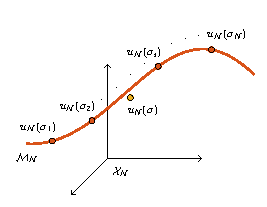
\includegraphics[width=0.6\textwidth]{figures/rb.pdf}
    \caption[%
    Skizze zur Motivation der Reduzierte-Basis-Methode.
    ]{
        Beispiel der Funktionsweise der Reduzierte"=Basis"=Methode im Falle eines eindimensionalen Parameters $\sigma$.
        Die Reduzierte"=Basis"=Lösungen $u_{N}(\sigma)$ ergeben sich als Linearkombinationen der Truth"=Lösungen $u_{\mathcal N}(\sigma_{i})$ für gewisse $\sigma_{i} \in \mathcal P$.
        }
    \label{figure:rbm_loesungsmenge}
\end{figure}

Wir beenden an dieser Stelle die Motivation, widmen uns nun einer rigorosen Einführung der Reduzierte"=Basis"=Methode und beginnen diese mit der Definition der grundlegenden Begriffe.

\begin{Definition}
\label{definition:rb_variationsproblem}
    Seien $N \in \mathbb{N}$ sowie $\mathcal S_{N} := \Set{ \bm \sigma_{1}, \dots, \bm \sigma_{N} } \subset \mathcal P$ eine Teilmenge der Parameter und $\Phi_{N} := \Set{ u_{\mathcal N}(\bm \sigma_{1}), \dots, u_{\mathcal N}(\bm \sigma_{N})} \subset \mathcal X_{\mathcal N}$ eine Basis, die durch die zugehörigen Truth-Lösungen gegeben sei.
    Seien weiter $\mathcal X_{N} := \spn \Phi_{N}$ und $\mathcal Y_{N} \subset \mathcal Y_{\mathcal N}$ ein $N$-dimensionaler Unterraum.
    Als \emph{Reduzierte"=Basis"=Variationsformulierung} von \cref{eq:diskretes_abstraktes_parametrisches_vp} bezeichnen wir das folgende Variationsproblem:
    \begin{equation}
    \label{eq:rb_abstraktes_parametriches_vp}
        \text{Sei } \bm \sigma \in \mathcal P, \text{ finde } u_{N}(\bm \sigma) \in \mathcal X_{N} \colon \quad b(u_{N}(\bm \sigma), v; \bm \sigma) = f(v) \quad \fa v \in \mathcal Y_{N}.
    \end{equation}
    Fernen nennen wir $u_{N}(\bm \sigma)$ \emph{Reduzierte"=Basis"=Lösung}.
\end{Definition}

Wie auch bei den Petrov"=Galerkin"=Verfahren muss sichergestellt werden, dass es sich bei dieser Diskretisierung tatsächlich um ein korrekt gestelltes Problem handelt.
Dies kann hauptsächlich durch die Wahl des Testraumes $\mathcal Y_{N}$ gesteuert werden.
An dieser Stelle nehmen wir an, dass dies stets bewerkstelligt werden kann.
Ein konkretes Verfahren, um diese zu wählen, geben wir an späterer Stelle an, wobei die Korrektheit im Rahmen dieser Arbeit nicht bewiesen werden kann und nur numerisch bekräftigt werden wird.

Weiter wollen wir begründen, warum wir eine Galerkin"=Diskretisierung als Grundlage verwenden und nicht das stetige Variationsproblem \cref{eq:abstraktes_parametrische_vp}.
Die zugrundeliegende Prämisse ist, neben der Berechenbarkeit, dass nach \cref{satz:lemma_von_cea}, unter gewissen Annahmen, die Petrov"=Galerkin"=Lösung $u_{\mathcal N}(\bm \sigma)$ die exakte Lösung $u(\bm \sigma)$ durch Verfeinerung der Diskretisierung beliebig gut approximieren kann.
Betrachten wir die Abschätzung
\begin{equation}
    \norm{u(\bm \sigma) - u_{N}(\bm \sigma)}_{\mathcal X} \leq \norm{u(\bm \sigma) - u_{\mathcal N}(\bm \sigma)}_{\mathcal X} + \norm{u_{\mathcal N}(\bm \sigma) - u_{N}(\bm \sigma)}_{\mathcal X},
\end{equation}
dann sagt dies gerade aus, dass der erste Summand beliebig klein gehalten werden kann, weswegen wir uns in diesem Kapitel lediglich für den zweiten Summanden, also den Fehler zwischen Truth- und Reduzierte"=Basis"=Lösung, interessieren.

Um die notationelle Wiederholung möglichst gering zu halten, seien für den Rest dieses Abschnitts stets durch $u_{N}(\bm \sigma) \in \mathcal X_{N}$ die Reduzierte-Basis-Lösung und durch $u_{\mathcal N}(\bm \sigma) \in \mathcal X_{\mathcal N}$ die Truth-Lösung zu einem Parameter $\bm \sigma \in \mathcal P$ gegeben.

Da es sich bei der Reduzierte"=Basis"=Diskretisierung um ein Galerkin"=Verfahren handelt, erhalten wir Analoga der Aussagen \cref{satz:galerkin_stabilitaet}, \cref{lemma:galerkin_orthogonalitaet} und \cref{satz:lemma_von_cea}, wobei die Truth-Räume die Rolle der stetigen Räume einnehmen.
An dieser Stelle wiederholen wir nur die Galerkin"=Orthogonalität ohne Beweis, da diese nachfolgend verwendet wird.

\begin{Lemma}
    \label{lemma:rb_galerkin_orthogonalitaet}
    Es gilt $b(u_{N}(\bm \sigma) - u_{\mathcal N}(\bm \sigma), v) = 0$ für alle $v \in \mathcal Y_{N}$, das heißt, der Fehler $u_{N}(\bm \sigma) - u_{\mathcal N}(\bm \sigma)$ ist orthogonal zu $\mathcal Y_{N}$.
\end{Lemma}

Den Fehler des vorherigen Lemmas finden wir auch in der nachfolgenden Definition, welche einen weiteren Baustein für die Reduzierte"=Basis"=Methode liefert.

\begin{Definition}
\label{definition:rbm_fehler_und_residuum}
    Als \emph{Fehler} $e_{N}(\bm \sigma) \in \mathcal X_{\mathcal N}$ bezeichnen wir
    \begin{equation}
        e_{N}(\bm \sigma) := u_{\mathcal N}(\bm \sigma) - u_{N}(\bm \sigma).
    \end{equation}
    Weiter sei das \emph{Residuum} $r_{N}(\blank; \bm \sigma) \colon \mathcal Y_{\mathcal N} \to \mathbb{R}$ festgelegt als
    \begin{equation}
    \label{eq:variationsproblem_residuum}
        r_{N}(v; \bm \sigma) := b(e_{N}(\bm \sigma), v; \bm \sigma), \quad v \in \mathcal Y_{\mathcal N}.
    \end{equation}
\end{Definition}

\begin{Lemma}
\label{lemma:rbm_residuum_ist_funktional}
    Das Residuum $r_{N}(\blank; \bm \sigma)$ ist für alle $\bm \sigma \in \mathcal P$ ein stetiges lineares Funktional, kurz also $r_{N}(\blank; \bm \sigma) \in \mathcal Y_{\mathcal N}'$.

    \begin{Beweis}
        Sowohl Linearität als auch Stetigkeit sind direkt ersichtlich, denn das Residuum kann nach Definition geschrieben werden als
        \begin{equation}
            \begin{aligned}
            r_{N}(v; \bm \sigma)
            &= b(e_{N}(\bm \sigma), v; \bm \sigma)
            = b(u_{\mathcal N}(\bm \sigma), v; \bm \sigma) - b(u_{N}(\bm \sigma), v; \bm \sigma)
            \\&= f(v) - b(u_{N}(\bm \sigma), v; \bm \sigma).
            \end{aligned}
        \end{equation}
    \end{Beweis}
\end{Lemma}

Das Residuum lässt sich nun verwenden, um eine der wichtigsten Eigenschaften der Reduzierte"=Basis"=Methoden herzuleiten, die Zertifizierung der Lösung durch eine a posteriori-Fehlerabschätzung.
Dazu benötigen wir eine untere Schranke $\beta_{\mathrm{LB}}(\bm \sigma)$ der inf-sup-Konstante $\beta_{\mathcal N}(\bm \sigma)$, da die exakte Konstante im Allgemeinen nicht bestimmt werden kann.

\begin{Lemma}
\label{lemma:rbm_fehler_schranke}
    Sei $\beta_{\mathrm{LB}}(\bm \sigma) > 0$ eine berechenbare untere Schranke für $\beta_{\mathcal N}(\bm \sigma)$.
    Dann gilt
    \begin{equation}
        \norm{u_{\mathcal N}(\bm \sigma) - u_{N}(\bm \sigma)}_{\mathcal X} \leq \Delta_{N}(\bm \sigma) := \frac{\norm{r_{N}(\blank; \bm \sigma)}_{\mathcal Y_{\mathcal N}'}}{\beta_{\mathrm{LB}}(\bm \sigma)},
    \end{equation}
    wobei wir $\Delta_{N}(\bm \sigma)$ als \emph{a posteriori-Fehlerschätzer} bezeichnen.

    \begin{Beweis}
        Wir können \cref{eq:variationsproblem_residuum} als Variationsproblem \cref{eq:diskretes_abstraktes_parametrisches_vp} auffassen, welches unter den getroffenen Annahmen die eindeutige Lösung $e_{N}(\bm \sigma)$ besitzt.
        Die Abschätzung folgt nun aus \cref{satz:galerkin_stabilitaet}.
    \end{Beweis}
\end{Lemma}

Dieser a posteriori-Fehlerschätzer bildet das Herzstück der Reduzierte"=Basis"=Methode, da er sowohl für die Konstruktion der niedrigdimensionalen Räume $\mathcal X_{N}$ und $\mathcal Y_{N}$, als auch für die bereits angesprochene Zertifizierung verwendet wird, welche eine garantierte obere Schranke zwischen Truth- und Reduzierte"=Basis"=Lösung liefert.
Wir sind bisher nicht darauf eingegangen, wie dieser Fehlerschätzer numerisch bestimmt werden kann.
Auf den ersten Blick scheint dies schwierig, da sowohl die Norm des Residuums als auch eine untere Schranke für die inf-sup-Konstante im Allgemeinen nur unter hohem Aufwand bestimmt werden können.
Diesem Punkt widmen wir uns im nächsten Abschnitt.

% TODO: eventuell was zur Effektivität sagen?
% Weiter wollen wir an dieser Stelle einen weiteren, auf den a posteriori-Fehlerschätzer aufbauenden, Begriff einführen.
% Dieser liefert ein Maß für die Güte des Fehlerschätzers.

% \begin{Lemma}
%     Die \emph{Effektivität} $\eta_{N}(\bm \sigma)$ des a posteriori-Fehlerschätzers ist beschränkt durch
%     \begin{equation}
%         h_{N}(\bm \sigma) := \frac{\Delta_{N}(\bm \sigma)}{\norm{u_{N}(\bm \sigma) - u_{\mathcal N}(\bm \sigma)}} \leq \frac{\gamma_{b}(\bm \sigma)}{\beta_{\mathrm{LB}}(\bm \sigma)}.
%     \end{equation}

%     \begin{Beweis}
%         TODO
%     \end{Beweis}
% \end{Lemma}




\section{Numerische Umsetzung} % (fold)
\label{sub:grb:rb:numerische_umsetzung}

Die numerische Umsetzung besteht aus mehreren Teilen, welche wir im Folgenden beschreiben werden.

\subsection{Zerlegung in Offline- und Online-Phase} % (fold)
\label{sub:zerlegung_in_offline_und_online_phase}

\begin{algorithm}[tb]
    \DontPrintSemicolon
    \SetKwInOut{Input}{Eingabe}\SetKwInOut{Output}{Ausgabe}
    \SetKwProg{Proc}{Prozedur}{}{}
    %
    \Input{Menge $\Xi_{\mathrm{train}} \subset \mathcal P$ der Trainingsparameter und Fehlertoleranz $\epsilon_{\mathrm{tol}} > 0$}
    \Output{Reduzierte-Basis-Ansatzraum $\mathcal X_{N}$ der Dimension $N$}
    \BlankLine
    Setze $N = 0$, $\mathcal P_{0} = \Set{}$, $\Phi_{0} = \Set{}$, $\mathcal X_{0} = \Set{0}$\;
    \While{$\max_{\bm \sigma \in \Xi_{\mathrm{train}}} \Delta_{N}(\bm \sigma) > \epsilon_{\mathrm{tol}}$}{
        $\bm \sigma_{N + 1} \leftarrow \arg \max_{\bm \sigma \in \Xi_{\mathrm{train}}} \Delta_{N}(\bm \sigma)$\;
        $\mathcal P_{N + 1} \leftarrow \mathcal P_{N} \cup \Set{\bm \sigma_{N + 1}}$\;
        $\Phi_{N + 1} \leftarrow \Phi_{N} \cup \Set{u_{\mathcal N}(\bm \sigma_{N + 1})}$\;
        $\mathcal X_{N + 1} \leftarrow \spn \Phi_{N + 1}$\;
        $N \leftarrow N + 1$\;
    }
    %
    \caption{Greedy Training}
    \label{algorithm:greedy_training}
\end{algorithm}

% subsection zerlegung_in_offline_und_online_phase (end)

\subsection{Bestimmung des Fehlerschätzers} % (fold)
\label{sub:bestimmung_des_fehlersch_tzers}

\begin{algorithm}[tb]
    \DontPrintSemicolon
    \SetKwInOut{Input}{Eingabe}\SetKwInOut{Output}{Ausgabe}
    \SetKwProg{Proc}{Prozedur}{}{}
    %
    \Input{Menge $\Xi_{\mathrm{train}} \subset \mathcal P$ der Trainingsparameter und Fehlertoleranz $\epsilon_{\mathrm{tol}} > 0$}
    \Output{Reduzierte-Basis-Ansatzraum $\mathcal X_{N}$}
    \BlankLine
    Setze $K = 1$, $\mathcal C_{1} = \Set{\bm \sigma_{1}}$ mit zufälligem $\bm \sigma_{1} \in \Xi_{\mathrm{train}}$\;
    \While{$\max_{\bm \sigma \in \Xi_{\mathrm{train}}} [(\beta_{\mathrm{UB}}(\bm \sigma; \mathcal C_{K}) - \beta_{\mathrm{LB}}(\bm \sigma; \mathcal C_{K})) / {\beta_{\mathrm{UB}}(\bm \sigma; \mathcal C_{K})}] > \epsilon_{\mathrm{tol}}$}{
        $\bm \sigma_{K + 1} \leftarrow \arg \max_{\bm \sigma \in \Xi_{\mathrm{train}}} [(\beta_{\mathrm{UB}}(\bm \sigma; \mathcal C_{K}) - \beta_{\mathrm{LB}}(\bm \sigma; \mathcal C_{K})) / {\beta_{\mathrm{UB}}(\bm \sigma; \mathcal C_{K})}]$\;
        $\mathcal C_{K + 1} \leftarrow \mathcal C_{K} \cup \Set{\bm \sigma_{K + 1}}$\;
        $K \leftarrow K + 1$\;
    }
    %
    \caption{Successive Constraint Method}
    \label{algorithm:scm_greedy}
\end{algorithm}

% subsection bestimmung_des_fehlersch_tzers (end)

\end{document}
